\documentclass[conference]{IEEEtran}
\IEEEoverridecommandlockouts
\usepackage{cite}
\usepackage{amsmath,amssymb,amsfonts}
\usepackage{graphicx}
\usepackage{textcomp}
\usepackage{xcolor}
\usepackage{booktabs}
\usepackage{multirow}
\usepackage{makecell}
\usepackage{tikz}
\usetikzlibrary{arrows.meta,positioning,fit,calc,backgrounds}
\usepackage[hidelinks]{hyperref}

\newcommand{\pt}{\,pt}
\newcommand{\ci}[2]{[$#1$, $#2$]}
\definecolor{snnblue}{HTML}{2A78D6}
\definecolor{frozengray}{HTML}{EFEEEA}
\definecolor{trainblue}{HTML}{E3EEFB}
\definecolor{calorange}{HTML}{FCE6DC}

\begin{document}

\title{Calibrated Concept Bottleneck Models on a Frozen Spiking Vision Backbone: A Controlled Comparison with Capacity-Matched ANNs}

\author{
\IEEEauthorblockN{P.~Manikanta}
\IEEEauthorblockA{\textit{[Department]} \\
\textit{[Institution]}\\
{[City]}, India \\
{[email]}}
\and
\IEEEauthorblockN{Ch.~Bhargav}
\IEEEauthorblockA{\textit{[Department]} \\
\textit{[Institution]}\\
{[City]}, India \\
{[email]}}
\and
\IEEEauthorblockN{Govardhan}
\IEEEauthorblockA{\textit{[Department]} \\
\textit{[Institution]}\\
{[City]}, India \\
{[email]}}
\and
\IEEEauthorblockN{K.~Deekshith}
\IEEEauthorblockA{\textit{[Department]} \\
\textit{[Institution]}\\
{[City]}, India \\
{[email]}}
}

\maketitle

\begin{abstract}
Concept bottleneck models (CBMs) predict human-readable concepts before the class, so decisions can be inspected and corrected; spiking neural networks (SNNs) compute with sparse binary events and promise energy-efficient inference. We build, to our knowledge, the first CBM on a spiking vision backbone and test it against capacity-matched artificial neural network (ANN) controls. A gated recurrent unit (GRU) reads the spike train of a frozen, ImageNet-pretrained SpikingResformer-Ti ($T=4$) step by step, a linear layer predicts 112 CUB-200-2011 attributes, and the 200-way class head sees only these concepts; per-concept Platt scaling calibrates them. Over five seeds the spiking CBM reaches 58.63\% test accuracy, statistically indistinguishable from a frozen ResNet-34 with an MLP decoder of the same 1.97\,M trainable-parameter budget (58.51\%; paired gap $+0.12$ points, 95\% CI [$-0.92$, $+1.17$]) and 2.4 points above a capacity-matched ResNet-18, at 5.7$\times$ lower estimated compute energy. Decoding the spikes in temporal order adds 1.1 points over a time-shuffled decoder, and calibration lowers the concept expected calibration error from 0.080 to 0.018 without a significant accuracy cost and raises accuracy after correcting 25\% of the concepts by 6.3 points. We also report what does not hold: the ANN's raw concepts are better (AUC 0.932 vs.\ 0.917) and benefit almost as much from calibration; memory traffic erases the advantage off chip, and also on chip at 8-bit precision; fewer time steps cost 2.3--7.6 points; under VLG-CBM's sparse-head protocol our concepts do not beat a size-matched random layer; and low-confidence predictions change under imperceptible input perturbations.
\end{abstract}

\begin{IEEEkeywords}
spiking neural networks, concept bottleneck models, interpretability, calibration, energy efficiency, fine-grained classification
\end{IEEEkeywords}

%% ------------------------------------------------------------------------------------------------
\section{Introduction}

Deep networks classify images accurately but rarely say why. For decisions that people must check, models that are interpretable by construction are preferable to explanations added afterwards~\cite{rudin2019stop}. Concept bottleneck models (CBMs)~\cite{koh2020concept} make the reason explicit: the network first predicts human-readable concepts, such as \emph{wing color: black}, and then predicts the class from those concepts only. A user can read the concepts behind each decision and correct a wrong one at test time (intervention).

Spiking neural networks (SNNs)~\cite{maass1997networks,roy2019towards} process information as binary spikes over a few time steps. A spike either triggers an addition or nothing, so SNNs replace most multiply--accumulate (MAC) operations with cheaper accumulates (ACs); this is the basis of their energy claims on event-driven hardware~\cite{davies2018loihi}. Spiking transformers and residual networks now exceed 74\% ImageNet top-1 accuracy~\cite{zhou2023spikformer,yao2023spike,shi2024spikingresformer}. Explanations of SNNs, however, have so far been post-hoc attribution maps~\cite{kim2021visual,bitar2023gradient,nguyen2023feature}; we are not aware of a concept bottleneck built on a spiking backbone.

Combining the two raises four questions that a fair evaluation must answer. \textbf{(Q1)}~Can concepts read from a frozen SNN support a classifier as accurate as an ANN with the same trainable capacity? \textbf{(Q2)}~Does the temporal structure of the spike train carry concept information beyond firing rates? \textbf{(Q3)}~Are the predicted concept probabilities calibrated well enough to show to a user and to support intervention? \textbf{(Q4)}~Does the energy advantage survive when memory traffic is counted~\cite{dampfhoffer2023snns}? Answering them requires controls that SNN comparisons often omit: equal trainable parameters, identical data augmentation, several seeds, paired statistical tests, and energy accounting beyond operation counts.

We attach a CBM to the frozen SpikingResformer-Ti backbone of Shi \emph{et al.}~\cite{shi2024spikingresformer} (our first base paper), evaluate it with the protocols of Koh \emph{et al.}~\cite{koh2020concept} and of VLG-CBM~\cite{srivastava2024vlgcbm} (our second base paper), and compare it with capacity-matched ResNet controls on CUB-200-2011~\cite{wah2011cub}. Our contributions are:
\begin{itemize}
\item A spiking CBM in which a GRU decodes the spike train of the last spiking layer step by step, a linear layer predicts 112 concepts, and a linear head predicts the class from the concepts only, with per-concept Platt calibration (Section~\ref{sec:method}).
\item A controlled comparison with ANN CBMs that have the same 1.97\,M trainable parameters, the same augmented views and three to five seeds, using paired bootstrap, McNemar and equivalence tests (Sections~\ref{sec:setup}--\ref{sec:results}).
\item Ablations that isolate spike timing, an evaluation under VLG-CBM's sparse-layer protocol, and an energy analysis that adds first-order memory traffic to operation counts.
\item An explicit account of negative results, including a stability test showing that low-confidence predictions change under imperceptible input noise.
\end{itemize}
In short, the answers are: Q1, yes in the sense that the accuracy is statistically indistinguishable from ResNet-34 (with five seeds, equivalence within $\pm$1 point holds over seeds and narrowly misses over test images); Q2, yes, but modestly: on static images, order adds about one point; Q3, yes, but calibration helps the ANN almost as much; Q4, only for compute alone or under optimistic on-chip memory assumptions, not with off-chip DRAM, and not at all once arithmetic and memory share one 8-bit precision.

%% ------------------------------------------------------------------------------------------------
\section{Related Work}

\textbf{Concept bottleneck models.} Koh \emph{et al.}~\cite{koh2020concept} introduced CBMs and test-time intervention, using 112 CUB attributes. Concept embedding models~\cite{espinosa2022concept} learn concept embeddings and train with random interventions; post-hoc CBMs~\cite{yuksekgonul2023posthoc} attach concepts to a frozen backbone; label-free CBMs~\cite{oikarinen2023labelfree} obtain concepts from a language model and CLIP; probabilistic CBMs~\cite{kim2023probabilistic} model concept uncertainty. Soft concept scores can leak class information that the concept names do not describe~\cite{margeloiu2021concept,mahinpei2021promises,havasi2022addressing}. VLG-CBM~\cite{srivastava2024vlgcbm} grounds language-model concepts with an open-vocabulary detector and proposes the number of effective concepts (NEC), a sparse final layer that limits such leakage. We follow Koh \emph{et al.} for concepts and joint training and VLG-CBM for the sparse-layer evaluation.

\textbf{Spiking vision backbones.} Deep SNNs are trained with surrogate gradients~\cite{neftci2019surrogate}, for example in SpikingJelly~\cite{fang2023spikingjelly}. Spikformer~\cite{zhou2023spikformer} and the Spike-driven Transformer~\cite{yao2023spike} brought self-attention to SNNs. SpikingResformer~\cite{shi2024spikingresformer} combines a ResNet-style multi-stage design with dual spike self-attention (DSSA) and group-wise spiking feed-forward networks; its 11.1\,M-parameter Ti variant reaches 74.34\% ImageNet top-1 at $T=4$. We use it as a frozen feature extractor.

\textbf{Explaining SNNs.} Spike activation maps based on inter-spike intervals~\cite{kim2021visual} and gradient- or spike-based attribution~\cite{bitar2023gradient,nguyen2023feature} highlight input regions after the fact. Our model is interpretable by construction: the class depends only on named concepts.

\textbf{Calibration and energy.} Modern networks are often miscalibrated~\cite{guo2017calibration}; Platt scaling~\cite{platt1999probabilistic} recalibrates scores and the expected calibration error (ECE)~\cite{naeini2015obtaining} measures the remaining gap. SNN energy is usually estimated from operation counts with 45\,nm costs, 4.6\,pJ per 32-bit MAC and 0.9\,pJ per AC~\cite{horowitz2014computing,shi2024spikingresformer}; hardware-aware studies show that memory access and neuron-state storage can remove the advantage~\cite{dampfhoffer2023snns}. We report both views.

%% ------------------------------------------------------------------------------------------------
\begin{figure*}[t]
\centering
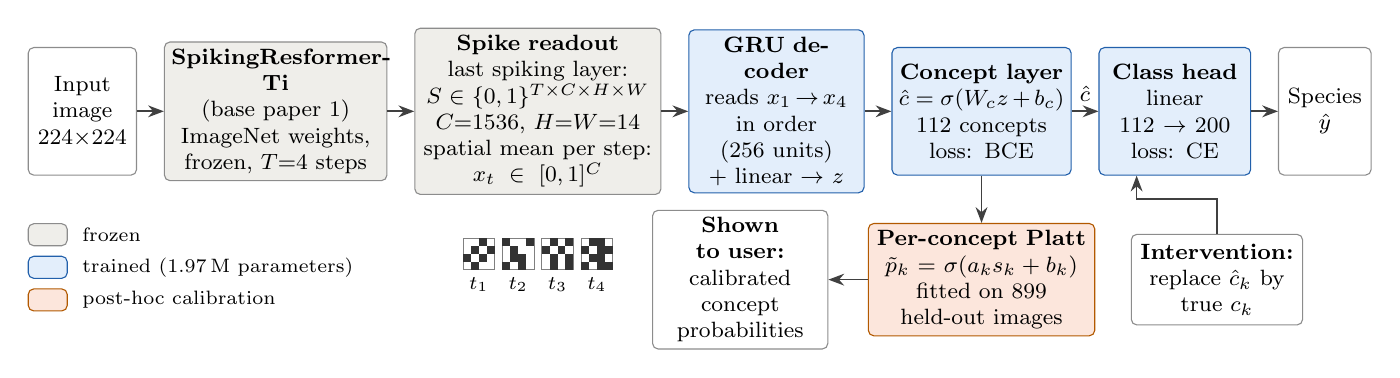
\begin{tikzpicture}[
  font=\footnotesize,
  box/.style={draw, rounded corners=2pt, align=center, minimum height=1.62cm, inner sep=2.5pt},
  frozen/.style={box, fill=frozengray, draw=black!45},
  train/.style={box, fill=trainblue, draw=snnblue!80!black},
  cal/.style={box, fill=calorange, draw=orange!70!black, minimum height=1.15cm},
  plain/.style={box, draw=black!45},
  arr/.style={-{Stealth[length=2mm]}, semithick, draw=black!75},
  node distance=0.34cm
]
\node[plain, text width=1.2cm] (img) {Input\\image\\$224{\times}224$};
\node[frozen, text width=2.65cm, right=of img] (bb) {\textbf{SpikingResformer-Ti}\\(base paper 1)\\ImageNet weights,\\frozen, $T{=}4$ steps};
\node[frozen, text width=2.95cm, right=of bb] (tap) {\textbf{Spike readout}\\last spiking layer:\\$S\in\{0,1\}^{T\times C\times H\times W}$\\$C{=}1536$, $H{=}W{=}14$\\spatial mean per step:\\$x_t\in[0,1]^{C}$};
\node[train, text width=2.05cm, right=of tap] (gru) {\textbf{GRU decoder}\\reads $x_1\!\to\!x_4$\\in order (256 units)\\+ linear $\to z$};
\node[train, text width=2.1cm, right=of gru] (cbl) {\textbf{Concept layer}\\$\hat c=\sigma(W_c z+b_c)$\\112 concepts\\loss: BCE};
\node[train, text width=1.75cm, right=of cbl] (head) {\textbf{Class head}\\linear\\$112\to200$\\loss: CE};
\node[plain, text width=1.0cm, right=of head] (out) {Species\\$\hat y$};
\draw[arr] (img) -- (bb);
\draw[arr] (bb) -- (tap);
\draw[arr] (tap) -- (gru);
\draw[arr] (gru) -- (cbl);
\draw[arr] (cbl) -- node[above]{$\hat c$} (head);
\draw[arr] (head) -- (out);
% second row
\node[cal, text width=2.7cm, below=0.6cm of cbl] (platt) {\textbf{Per-concept Platt}\\$\tilde p_k=\sigma(a_k s_k+b_k)$\\fitted on 899 held-out images};
\node[plain, text width=2.05cm, minimum height=1.15cm, left=0.5cm of platt] (user) {\textbf{Shown to user:}\\calibrated concept\\probabilities};
\node[plain, text width=2.0cm, minimum height=1.15cm, right=0.45cm of platt] (int) {\textbf{Intervention:}\\replace $\hat c_k$ by\\true $c_k$};
\draw[arr] (cbl) -- (platt);
\draw[arr] (platt) -- (user);
\draw[arr] (int.north) |- ($(head.south west)!0.5!(head.south)+(0,-0.3)$) -- ($(head.south west)!0.5!(head.south)$);
% spike raster icon under the readout node
\begin{scope}[shift={($(tap.south)+(-0.95,-0.95)$)}]
  \foreach \t/\pat in {0/{1,4,6,9,11,14}, 1/{0,2,5,6,9,12,15}, 2/{1,3,5,7,8,10,13,15}, 3/{0,2,3,5,6,8,10,11,13,14}} {
    \begin{scope}[shift={(\t*0.5,0)}]
      \draw[black!50, line width=0.3pt] (0,0) rectangle (0.4,0.4);
      \foreach \c in \pat { \pgfmathtruncatemacro{\rr}{int(\c/4)}\pgfmathtruncatemacro{\qq}{mod(\c,4)}
        \fill[black!80] (\qq*0.1,\rr*0.1) rectangle ++(0.1,0.1); }
      \node[font=\scriptsize, below=-0.03cm] at (0.2,0) {$t_{\the\numexpr\t+1\relax}$};
    \end{scope}
  }
\end{scope}
% legend
\node[frozen, minimum height=0.28cm, text width=0.32cm, anchor=west] (lf) at ($(img.south west)+(0,-0.75)$) {};
\node[right=0.06cm of lf, font=\scriptsize] {frozen};
\node[train, minimum height=0.28cm, text width=0.32cm, below=0.12cm of lf] (lt) {};
\node[right=0.06cm of lt, font=\scriptsize] {trained (1.97\,M parameters)};
\node[cal, minimum height=0.28cm, text width=0.32cm, below=0.12cm of lt] (lc) {};
\node[right=0.06cm of lc, font=\scriptsize] {post-hoc calibration};
\end{tikzpicture}
\caption{The spiking concept bottleneck model. A frozen SpikingResformer-Ti looks at the image for four time steps; the binary spikes of its last spiking layer are averaged over space at each step and read in order by a GRU. The concept layer predicts 112 CUB attributes and the class head sees only these concepts. Per-concept Platt scaling, fitted on held-out images, turns raw concept scores into calibrated probabilities for display; intervention replaces predicted concepts with true values before the head.}
\label{fig:model}
\end{figure*}

\section{Method}\label{sec:method}

Fig.~\ref{fig:model} shows the model. Only the decoder, the concept layer and the class head are trained.

\subsection{Frozen spiking backbone and spike readout}
Each $224{\times}224$ image is presented to SpikingResformer-Ti~\cite{shi2024spikingresformer} for $T=4$ time steps. Its leaky integrate-and-fire (LIF) neurons follow
\begin{equation}
\begin{aligned}
H_t &= V_{t-1} + \tfrac{1}{\tau}\big(X_t - (V_{t-1}-V_r)\big),\\
S_t &= \Theta(H_t - V_{\mathrm{th}}),\qquad V_t = H_t\,(1-S_t) + V_r S_t ,
\end{aligned}
\label{eq:lif}
\end{equation}
with $\tau=2$, $V_{\mathrm{th}}=1$, $V_r=0$, input current $X_t$ and the Heaviside step $\Theta$. All backbone weights come from the authors' ImageNet checkpoint and stay frozen. We read the binary spikes $S\in\{0,1\}^{T\times C\times H\times W}$ of the LIF layer that feeds the final down-projection of the last group-wise feed-forward block ($C=1536$, $H=W=14$), the last spiking layer before global pooling. A patched neuron step records $S$ without changing the computation: on 32 test images it reproduces the native SpikingJelly neuron exactly (0 of $3.85\times10^{7}$ spike values differ; identical backbone outputs). Averaging over space gives one rate vector per step,
\begin{equation}
x_t=\frac{1}{HW}\sum_{h,w} S_{t,:,h,w}\in[0,1]^{C},\qquad t=1,\dots,T .
\label{eq:pool}
\end{equation}
In preliminary linear-probe experiments, the membrane potentials of the same layer gave mixed results against spike rates (slightly better without regularization, slightly worse with strong regularization), so the model reads spikes, which are also what spiking hardware communicates.

\subsection{Temporal decoder, concept layer and class head}
A single-layer GRU~\cite{cho2014learning} with 256 hidden units reads $x_1,\dots,x_T$ in order, $h_t=\mathrm{GRU}(x_t,h_{t-1})$ with $h_0=0$, and a linear projection maps the last state back to the backbone width, $z=W_p h_T+b_p\in\mathbb{R}^{1536}$. The concept layer predicts concept logits $s=W_c z+b_c$ and probabilities $\hat c=\sigma(s)\in(0,1)^K$ for $K=112$ concepts, and the class head predicts $\hat y=\mathrm{softmax}(W_y\hat c+b_y)$ over 200 species. Because the head sees only $\hat c$, every class score is a linear function of named concepts. The trainable parameters are the GRU (1.378\,M), the projection (0.395\,M), the concept layer (0.172\,M) and the head (0.023\,M), 1.967\,M in total; the 11.1\,M backbone weights are not trained.

The model is trained jointly~\cite{koh2020concept} with
\begin{equation}
\mathcal{L}=\mathrm{BCE}(\hat c, c)+\mathrm{CE}(\hat y, y),
\label{eq:loss}
\end{equation}
where $c\in\{0,1\}^K$ are the concept labels and the BCE is averaged over concepts and images. During training, each concept passed to the head is replaced by its label with probability 0.25 (concept dropout), which exposes the head to corrected concepts, similar to the random-intervention training of~\cite{espinosa2022concept}.

\subsection{Per-concept calibration}
For each concept $k$ we fit Platt scaling~\cite{platt1999probabilistic},
\begin{equation}
\tilde p_k=\sigma(a_k s_k + b_k),
\label{eq:platt}
\end{equation}
by minimizing the negative log-likelihood on the 899 held-out training images plus a penalty $\lambda[(a_k-1)^2+b_k^2]/n$ ($\lambda=5$, $n=899$) that keeps rare concepts close to the identity map (300 Adam steps, learning rate 0.05). All fitted slopes $a_k$ are positive, so the ranking of images for each concept, and hence concept AUC, does not change. The calibrated probabilities are what a user sees. The class decision can either keep the raw $\hat c$ (display-only calibration, accuracy unchanged by construction) or use a head retrained on $\tilde p$ (Section~\ref{sec:interv}).

\subsection{Simulated intervention}
To simulate a user who corrects concepts, we replace a random subset containing a fraction $f\in\{0.1,0.25,0.5,0.75,1\}$ of the 112 head inputs with the true concept values and measure test accuracy, averaging over 10 random subsets per fraction that are shared by all models. No human study is involved.

\subsection{Energy model}\label{sec:energy-model}
Following~\cite{horowitz2014computing,shi2024spikingresformer}, a spike-driven synaptic operation costs one AC (0.9\,pJ) and every non-spiking operation one MAC (4.6\,pJ, 32-bit floating point, 45\,nm). For the SNN we count ACs from the spike activity measured on 160 test images and MACs for the non-spiking stem convolution, the GRU and its projection, the concept layer and the head. The backbone is truncated after the tapped layer, and the stateless stem (convolution, batch normalization, max pooling) is computed once and shared by the four steps, which gives identical spikes (0 of $6.98\times10^9$ differ) and identical predictions on all 5,794 test images. ANNs are charged one MAC per multiply--accumulate. Batch normalization, residual additions, pooling and neuron updates are not counted on either side. To include memory, we add a first-order count of the bytes each model reads and writes per image (8-bit weights read once, 8-bit activations, spikes as 1-bit maps, and a 16-bit membrane potential read and written for every neuron at every step) and charge them at Horowitz's per-access costs: 12.5\,pJ/B for a 1\,MB SRAM and 162.5--325\,pJ/B for off-chip DRAM~\cite{horowitz2014computing}. The model has no cache hierarchy and is not a hardware measurement.

%% ------------------------------------------------------------------------------------------------
\section{Experimental Setup}\label{sec:setup}

\textbf{Data.} CUB-200-2011~\cite{wah2011cub} has 11,788 images of 200 bird species (5,994 for training, 5,794 for testing). We use the 112 binary attributes of Koh \emph{et al.}~\cite{koh2020concept}, obtained by class-level majority voting over the training images, so all images of a species share one concept vector. A fixed random 15\% of the official training split (899 images) is held out for epoch selection and calibration; the other 5,095 images are used for training. The test split is used only for the final evaluation.

\textbf{Training.} Every model trains only its decoder, concept layer and head on features of a frozen backbone. Training images are augmented (random resized crop with scale 0.7--1.0, horizontal flip, color jitter 0.3/0.3/0.2). To make many runs affordable, eight augmented views per training image are precomputed once through every backbone, so all models see identical views, and one view per image is drawn in each epoch; held-out and test images are only resized. We use AdamW~\cite{loshchilov2019decoupled} (learning rate $10^{-3}$, weight decay $10^{-4}$), batch size 32, 50 epochs with a cosine schedule~\cite{loshchilov2017sgdr}, gradient clipping at 5 and concept dropout 0.25, with seeds 0, 1 and 2. We report the epoch with the best held-out class accuracy; selecting by held-out concept AUC gives the same conclusions for all decoder models.

\textbf{Baselines.} ANN controls use frozen ResNet-18, ResNet-34 and ResNet-50~\cite{he2016deep} pretrained on ImageNet~\cite{deng2009imagenet} (69.8\%, 73.3\% and 76.1\% top-1; SpikingResformer-Ti: 74.3\%). ``+\,MLP'' controls insert a $512\!\to\!1841\!\to\!512$ GELU MLP before the concept layer so that their trainable parameters equal those of the spiking model (1.97\,M, within 0.02\%); ``linear'' controls train only the concept layer and the head. SNN ablations keep the backbone and change the readout: a GRU trained on time steps randomly permuted per sample at every step (tested in natural order), a time-averaged MLP ($1536\!\to\!576\!\to\!1536$ on the mean of $x_t$, also 1.97\,M parameters), and a spike-rate readout without decoder.

\textbf{Metrics and statistics.} We report test accuracy, mean per-concept ROC AUC, and mean per-concept ECE with 15 equal-width bins~\cite{naeini2015obtaining}. Comparisons are paired: a bootstrap~\cite{efron1993introduction} over the 5,794 test images (10,000 resamples shared by all models and seeds; the three per-seed gaps are averaged within each resample), the exact McNemar test per seed~\cite{mcnemar1947note}, and two one-sided tests (TOST)~\cite{schuirmann1987comparison}, which declare equivalence when the 90\% bootstrap interval lies within $\pm$1 point for accuracy or $\pm$0.01 for AUC and ECE. Experiments ran on an NVIDIA RTX 3050 laptop GPU.

%% ------------------------------------------------------------------------------------------------
\begin{table*}[t]
\caption{Main results on CUB-200-2011 (5,794 test images, mean $\pm$ s.d.\ over three seeds, epoch selected on held-out class accuracy). Params: trainable parameters (decoder, concept layer and head). ECE cal.: after per-concept Platt scaling fitted on the held-out images. Bold: best value in each column.}
\label{tab:main}
\centering
\footnotesize
\setlength{\tabcolsep}{5pt}
\begin{tabular}{@{}llrcccc@{}}
\toprule
Model & Backbone and readout & Params & Accuracy (\%) $\uparrow$ & Concept AUC $\uparrow$ & ECE raw $\downarrow$ & ECE cal.\ $\downarrow$ \\
\midrule
\textbf{SNN + GRU (ours)} & SpikingResformer-Ti, GRU over $x_1\!\to\!x_4$ & 1.97\,M & 58.60 $\pm$ 0.20 & 0.917 $\pm$ 0.002 & 0.080 & 0.0177 \\
SNN + GRU, time-shuffled & same, steps permuted in training & 1.97\,M & 57.46 $\pm$ 0.24 & 0.914 $\pm$ 0.003 & 0.083 & 0.0183 \\
SNN + MLP, time-averaged & same, MLP on mean of $x_t$ & 1.97\,M & 56.47 $\pm$ 0.16 & 0.878 $\pm$ 0.000 & 0.106 & 0.0212 \\
SNN spike rate & same, no decoder & 0.19\,M & 45.65 $\pm$ 0.29 & 0.866 $\pm$ 0.000 & 0.119 & 0.0206 \\
\midrule
ResNet-18, linear & ResNet-18 (69.8\%) & 0.08\,M & 56.92 $\pm$ 0.51 & 0.850 $\pm$ 0.000 & 0.119 & 0.0206 \\
ResNet-18 + MLP & ResNet-18, MLP $512\!\to\!1841\!\to\!512$ & 1.97\,M & 56.24 $\pm$ 0.15 & 0.922 $\pm$ 0.001 & 0.076 & 0.0173 \\
ResNet-34, linear & ResNet-34 (73.3\%) & 0.08\,M & 59.07 $\pm$ 0.68 & 0.857 $\pm$ 0.000 & 0.121 & 0.0209 \\
\textbf{ResNet-34 + MLP} & ResNet-34, MLP $512\!\to\!1841\!\to\!512$ & 1.97\,M & 58.69 $\pm$ 0.78 & \textbf{0.932 $\pm$ 0.002} & \textbf{0.061} & \textbf{0.0168} \\
ResNet-50, linear & ResNet-50 (76.1\%) & 0.25\,M & \textbf{62.50 $\pm$ 0.33} & 0.873 $\pm$ 0.000 & 0.106 & 0.0206 \\
\bottomrule
\end{tabular}
\end{table*}

\begin{table}[t]
\caption{Paired differences (pooled over three seeds, bootstrap 95\% CI over test images). Accuracy in points; AUC and ECE are raw. All AUC and ECE intervals exclude zero and are narrower than $\pm$0.0021.}
\label{tab:paired}
\centering
\footnotesize
\setlength{\tabcolsep}{3pt}
\begin{tabular}{@{}lccc@{}}
\toprule
Comparison & $\Delta$Acc [95\% CI] & $\Delta$AUC & $\Delta$ECE \\
\midrule
\multicolumn{4}{@{}l}{\emph{SNN + GRU minus ANN control}}\\
\quad ResNet-34 + MLP & $-0.10$ \ci{-1.20}{+1.01} & $-0.0150$ & $+0.0195$ \\
\quad ResNet-18 + MLP & $+2.36$ \ci{+1.24}{+3.46} & $-0.0049$ & $+0.0045$ \\
\quad ResNet-34, linear & $-0.47$ \ci{-1.64}{+0.68} & $+0.0604$ & $-0.0408$ \\
\quad ResNet-50, linear & $-3.90$ \ci{-5.11}{-2.73} & $+0.0442$ & $-0.0255$ \\
\midrule
\multicolumn{4}{@{}l}{\emph{SNN + GRU minus SNN ablation}}\\
\quad time-shuffled GRU & $+1.14$ \ci{+0.61}{+1.66} & $+0.0032$ & $-0.0028$ \\
\quad \quad live augmentation & $+0.99$ \ci{+0.49}{+1.50} & $+0.0031$ & $-0.0038$ \\
\quad time-averaged MLP & $+2.13$ \ci{+1.35}{+2.91} & $+0.0399$ & $-0.0259$ \\
\midrule
\multicolumn{4}{@{}l}{\emph{Fewer time steps (GRU retrained) minus $T=4$}}\\
\quad $T=3$ & $-2.34$ \ci{-3.01}{-1.66} & $-0.0136$ & $+0.0079$ \\
\quad $T=2$ & $-7.61$ \ci{-8.53}{-6.67} & $-0.0408$ & $+0.0252$ \\
\bottomrule
\end{tabular}
\end{table}

\begin{figure}[t]
\centering
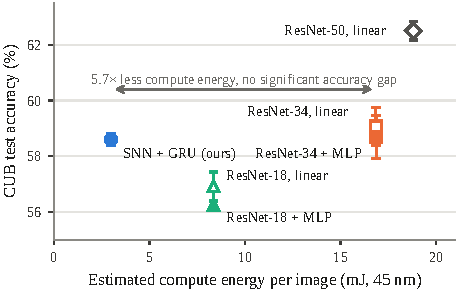
\includegraphics[width=\columnwidth]{figs/acc_energy.pdf}
\caption{Test accuracy (mean $\pm$ s.d., three seeds) against estimated compute energy per image. Filled markers: decoder with 1.97\,M trainable parameters; open markers: linear head.}
\label{fig:accenergy}
\end{figure}

\section{Results}\label{sec:results}

\subsection{Accuracy against capacity-matched ANNs (Q1)}
Table~\ref{tab:main} lists all models and Table~\ref{tab:paired} the paired tests. The spiking CBM reaches $58.60\pm0.20$\% and ResNet-34 + MLP $58.69\pm0.78$\%. The paired gap is $-0.10$ points (95\% CI [$-1.20$, $+1.01$]; McNemar $p=0.61$, 0.73 and 0.20 for the three seeds). Equivalence within $\pm$1 point is not established (TOST $p=0.054$): the 90\% interval supports a margin of 1.02 points over test images and 1.32 points over seeds. Two further seeds per model (3 and 4, trained on a CPU with the same recipe and views) give $58.63\pm0.36$\% for the spiking CBM and $58.51\pm0.68$\% for ResNet-34 + MLP, a paired gap of $+0.12$ points [$-0.92$, $+1.17$] (per-seed gaps $+0.38$, $+0.26$, $-0.93$, $+0.48$, $+0.43$). With five seeds, equivalence within $\pm$1 point holds over seeds (seed-level TOST $p=0.015$; margin 0.69 points) but still narrowly misses over test images (TOST $p=0.052$; margin 1.01 points). We therefore claim no significant difference and equivalence within about $\pm$1.0 point, not a strict match within one point. Selecting epochs by concept AUC gives the same picture ($+0.09$ [$-1.04$, $+1.22$]). The spiking CBM is 2.36 points [1.24, 3.46] more accurate than ResNet-18 + MLP (McNemar $p\le0.007$ on every seed) and not significantly different from the linear ResNet-34. The linear ResNet-50, whose backbone is 1.8 points better on ImageNet, is 3.90 points more accurate at 6.3$\times$ the compute energy (Fig.~\ref{fig:accenergy}).

Augmentation is essential for a fair comparison. Without it, decoder models overfit (SNN + GRU 48.03\%, ResNet-34 + MLP 55.25\%) while linear heads barely change, which made the ANNs look 5--10 points better in our earlier experiments.

\subsection{Does spike timing matter? (Q2)}\label{sec:timing}
The lower half of Table~\ref{tab:paired} isolates the readout. Reading the four steps in order beats the same GRU trained on randomly permuted steps by 1.14 points [0.61, 1.66], with higher concept AUC and lower ECE, on every seed. Without augmentation, time shuffling had acted as a regularizer and even helped, so we repeated this comparison with live augmentation, a fresh random view in every epoch for both runs of each seed: order still adds 0.99 points [0.49, 1.50] (60.06\% vs.\ 59.07\%; McNemar $p=0.026$, 0.026, 0.008). Trained with the same live views, recipe and selection, ResNet-34 + MLP reaches 58.08\% (56.01, 58.73, 59.51; 58.69\% with eight cached views), so the spiking model gains from live augmentation and the ANN does not: the spiking CBM is 1.98 points [0.86, 3.08] more accurate. This lead depends on the selection rule (one ANN seed selected an early epoch); with concept-AUC selection it is 1.02 points [$-0.08$, $+2.13$], not significant. We therefore conclude only that live augmentation does not favor the ANN. This effect is modest: the input is a static image, the steps come from the network's own dynamics, and each is spatially averaged, so it shows that internal spike order carries some concept information, not that the model uses temporal structure in data; event-camera input is the stronger test (Section~\ref{sec:disc}). Keeping per-step information also matters: a time-averaged MLP of equal size is 2.13 points [1.35, 2.91] less accurate with concept AUC lower by 0.040, and a readout without decoder reaches only 45.65\%. Finally, the time steps cannot simply be cut. Running the frozen backbone for $T=3$ or $T=2$ steps and retraining the decoder costs 2.34 and 7.61 points, so this backbone needs all four steps.

\begin{figure*}[t]
\centering
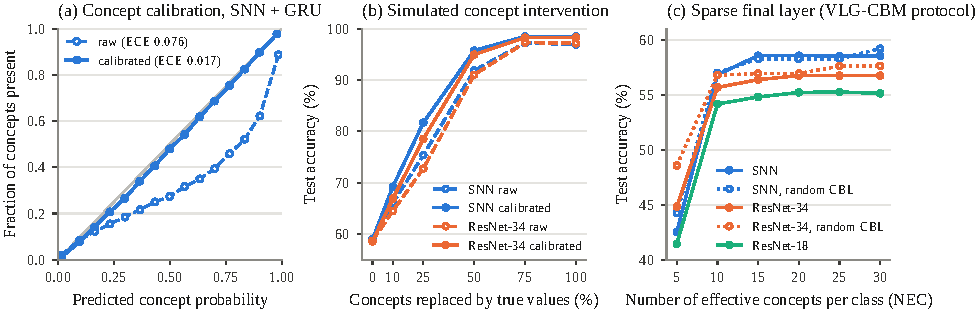
\includegraphics[width=\textwidth]{figs/calib_interv_nec.pdf}
\caption{(a) Reliability of the spiking CBM's concept probabilities (seed 0, all 112 concepts $\times$ 5,794 test images pooled): raw scores over-predict concept presence, per-concept Platt scaling removes most of the gap; ECE values are the mean over concepts. (b) Accuracy when a fraction of the head's concept inputs is replaced by true values (head retrained on raw or calibrated concepts, three seeds). (c) Accuracy of a sparse elastic-net final layer at a controlled number of effective concepts per class (VLG-CBM protocol); ``random CBL'' replaces the trained concept layer by 512 random features. The ResNets in (b) and (c) use the MLP decoder with the same 1.97\,M trainable-parameter budget as the spiking model.}
\label{fig:calib}
\end{figure*}

\subsection{Concept quality and calibration (Q3)}
The spiking model's concepts are better than those of ANN backbones without a decoder (AUC 0.917 vs.\ 0.850--0.873), but worse than ResNet-34 + MLP (0.932; gap $-0.0150$ [$-0.0170$, $-0.0129$]) and slightly below ResNet-18 + MLP (0.922; gap $-0.0049$, equivalent within $\pm$0.01). Raw concept probabilities are systematically too high: they over-predict that concepts are present (Fig.~\ref{fig:calib}a), with raw ECE 0.080 for the spiking model and 0.061 for ResNet-34 + MLP. Per-concept Platt scaling brings every model to 0.017--0.021 (Table~\ref{tab:main}) and leaves AUC unchanged (largest change $2\times10^{-6}$). After calibration the spiking model and ResNet-34 + MLP are equivalent within $\pm$0.01 (0.0177 vs.\ 0.0168; gap $+0.0009$ [$+0.0005$, $+0.0017$]). A single global Platt map reaches only 0.043, so per-concept parameters are needed.

\subsection{Intervention}\label{sec:interv}
We retrained the class head on raw or calibrated concepts (three seeds each) and corrected random concept subsets (Fig.~\ref{fig:calib}b). Calibration has no significant accuracy cost (spiking model $-0.12$ [$-0.45$, $+0.21$]; ResNet-34 + MLP $-0.16$ [$-0.45$, $+0.14$]) and makes corrections more effective. With 25\% of the concepts corrected, accuracy rises from 75.37\% to 81.69\% for the spiking model ($+6.32$ [6.04, 6.59]) and from 72.74\% to 78.53\% for ResNet-34 + MLP ($+5.80$ [5.55, 6.05]). The benefit is therefore not specific to the SNN; the SNN gains a small but significant 0.52 points [0.21, 0.83] more. With all concepts corrected both models reach 98.3--98.5\% on calibrated inputs. This is not a measure of interpretability: the labels are class-level and each of the 200 species has its own 112-concept vector, so correcting every concept gives the head the answer. Full intervention is an upper bound; partial correction (10--25\%) is the informative regime. In addition, the seed-averaged curves never drop by more than 0.5 points as more concepts are corrected. Feeding calibrated concepts to the jointly trained head without retraining costs 1.8 points (56.79\%), so in deployment calibration should be display-only unless the head is retrained.

\begin{table}[t]
\caption{Base paper 2 protocol: accuracy (\%) of a sparse final layer with NEC concepts per class (mean $\pm$ s.d., three seeds). ANEC-avg: mean over NEC 5--30. Top block: reported by VLG-CBM~\cite{srivastava2024vlgcbm} with a ResNet-18 fine-tuned on CUB, not like-for-like with our frozen backbones. ``Random ($n$)'': a random concept layer of $n$ features; 112 matches our concept layer (NEC\,=\,5 only).}
\label{tab:nec}
\centering
\footnotesize
\setlength{\tabcolsep}{3pt}
\begin{tabular}{@{}lccc@{}}
\toprule
Concept layer & ANEC-5 & ANEC-avg & Dense \\
\midrule
VLG-CBM (reported) & 75.79 & 75.82 & -- \\
LF-CBM (reported) & 53.51 & 69.11 & -- \\
Random baseline (reported) & 68.91 & 73.44 & -- \\
\midrule
SNN + GRU (ours) & 42.52 $\pm$ 0.74 & 55.58 $\pm$ 0.06 & 58.60 \\
SNN + GRU, random (512) & 44.25 $\pm$ 1.59 & 55.87 $\pm$ 0.65 & -- \\
SNN + GRU, random (112) & 43.91 $\pm$ 0.56 & -- & -- \\
ResNet-34 + MLP & 44.82 $\pm$ 0.95 & 54.50 $\pm$ 0.35 & 58.69 \\
ResNet-34 + MLP, random (512) & 48.56 $\pm$ 1.43 & 55.73 $\pm$ 0.25 & -- \\
ResNet-34 + MLP, random (112) & 47.78 $\pm$ 0.63 & -- & -- \\
ResNet-18 + MLP & 41.43 $\pm$ 1.23 & 52.66 $\pm$ 0.51 & 56.24 \\
\bottomrule
\end{tabular}
\end{table}

\subsection{Base paper 2: sparse final layer and NEC}
VLG-CBM~\cite{srivastava2024vlgcbm} evaluates CBMs with a sparse final layer whose number of effective concepts per class (NEC) is fixed, so that a dense head cannot hide information in many small weights. We reimplemented this protocol on our trained concept layers: concept logits standardized with training statistics, an elastic-net~\cite{zou2005regularization} multinomial head ($\alpha=0.99$, the default of the LF-CBM code that VLG-CBM builds on) along a 50-point regularization path solved with FISTA~\cite{beck2009fast} instead of GLM-SAGA~\cite{wong2021leveraging} (same objective), and pruning of the sparsest path point with at least NEC effective concepts to exactly NEC non-zero weights per class on average. At NEC\,=\,5 the spiking model reaches 42.52\%, below a random concept layer of 512 features treated the same way (44.25\%); the same holds for ResNet-34 + MLP (44.82\% vs.\ 48.56\%) (Table~\ref{tab:nec}, Fig.~\ref{fig:calib}c). The larger random layer is not the reason: a random layer with the same 112 features also wins, by 1.39 points [0.60, 2.19] for the spiking model, 2.96 [2.21, 3.73] for ResNet-34 + MLP and 3.35 [2.62, 4.07] for ResNet-18 + MLP. With five concepts per class, the human attributes as learned here are less useful than random projections of the same features for every backbone; the spiking model has the smallest deficit. The spiking model is below ResNet-34 + MLP at NEC\,=\,5 ($-2.30$ [$-3.34$, $-1.26$]) but above it at NEC\,=\,10 ($+1.16$ [0.06, 2.27]) and NEC\,=\,30 ($+1.80$ [0.68, 2.92]), and it is above ResNet-18 + MLP at every NEC. VLG-CBM's 75.79\% comes from a backbone fine-tuned on CUB and grounded concepts; the gap is likely due mainly to backbone training and the concept set (we did not test this), and the comparison is not like-for-like.

\subsection{Energy (Q4)}

\begin{table}[t]
\caption{Energy ratio ANN\,/\,SNN per image (above 1: the SNN uses less). SNN: 2.98\,mJ compute and 282\,MB of memory traffic (8-bit weights and activations, 16-bit membrane). Break-even: memory cost per byte at which both are equal. The SRAM column is a lower bound: neither model's weights fit in 1\,MB.}
\label{tab:energy}
\centering
\footnotesize
\setlength{\tabcolsep}{3.2pt}
\begin{tabular}{@{}lccccc@{}}
\toprule
Compared ANN & \makecell{Compute\\(mJ)} & \makecell{Compute\\only} & \makecell{+1\,MB\\SRAM} & \makecell{+DRAM\\162.5--325\,pJ/B} & \makecell{Break-\\even} \\
\midrule
Same arch., dense & 18.02 & 6.05$\times$ & 2.84$\times$ & 0.49--0.31$\times$ & 61.1 \\
ResNet-18 + MLP & 8.35 & 2.80$\times$ & 1.32$\times$ & 0.23--0.15$\times$ & 20.3 \\
ResNet-34 + MLP & 16.86 & 5.66$\times$ & 2.65$\times$ & 0.45--0.28$\times$ & 55.1 \\
ResNet-50, linear & 18.80 & 6.31$\times$ & 2.98$\times$ & 0.54--0.35$\times$ & 66.9 \\
\bottomrule
\end{tabular}
\end{table}

\begin{figure}[t]
\centering
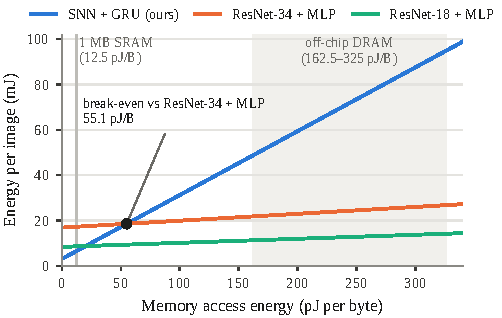
\includegraphics[width=\columnwidth]{figs/energy_memory.pdf}
\caption{Energy per image (compute plus memory traffic: 8-bit weights and activations, 16-bit membrane) as a function of the memory cost per byte. The spiking model moves 282\,MB per image, against 30\,MB for ResNet-34 + MLP, and loses its advantage above 55.1\,pJ/B.}
\label{fig:energy}
\end{figure}

The spiking CBM needs an estimated 2.98\,mJ per image ($2.67\times10^9$ ACs and $1.24\times10^8$ MACs); the neuron-weighted spike density over its 38 LIF layers is 17.5\%. This is 5.66$\times$ less than ResNet-34 + MLP (16.86\,mJ) and 6.05$\times$ less than the same architecture run as a dense ANN, which isolates the effect of spiking (Table~\ref{tab:energy}). Shi \emph{et al.} report 2.46\,mJ for the full Ti classifier under their counting; we apply one counting rule to all models, so the ratios are internally consistent.

Memory traffic changes the picture (Fig.~\ref{fig:energy}). The SNN moves 282\,MB per image, 60\% of it membrane potentials (169\,MB), against 30\,MB for ResNet-34 + MLP. If every byte cost as much as a 1\,MB SRAM access, the SNN would still use 2.65$\times$ less energy than ResNet-34 + MLP; this is a lower bound, since the 8-bit weights alone (10.2\,MB for the SNN, 21.3\,MB for ResNet-34) do not fit in 1\,MB, and a real design lies between this case and DRAM. With DRAM the SNN uses 2.24--3.54$\times$ more energy; the break-even memory cost is 55.1\,pJ/B. Assumed reductions of membrane traffic (8- or 4-bit membrane, on-chip buffers up to 8\,MiB) raise the break-even to at most 161.9\,pJ/B, still below the cheapest DRAM cost of 162.5\,pJ/B; even removing all membrane traffic, a bound rather than a design, only reaches parity there.

\textbf{One precision for arithmetic and memory.} The numbers above charge arithmetic at 32-bit floating-point cost but memory at 8 bits. With 32-bit arithmetic and 32-bit memory, the SNN still uses 1.78$\times$ less energy than ResNet-34 + MLP at 1\,MB-SRAM cost, but the break-even falls to 29.8\,pJ/B. With 8-bit arithmetic (0.2\,pJ per multiply; 0.03\,pJ per 8-bit or 0.1\,pJ per 32-bit addition~\cite{horowitz2014computing}) and 8-bit memory, the compute-only ratio is 3.6--7.8$\times$, depending on the accumulator width, but memory then dominates: the SNN uses 2.6--2.9$\times$ more energy than ResNet-34 + MLP already at 1\,MB-SRAM cost, and the break-even of 2.9--3.2\,pJ/B lies below any memory large enough to hold the weights. Under a consistent precision, the spiking model is cheaper only in arithmetic, not in total. Any energy benefit therefore needs neuromorphic-style hardware that keeps neuron state, and most weights, on chip~\cite{dampfhoffer2023snns,davies2018loihi}, and even then it is an estimate that has to be measured.

\subsection{Per-image stability}\label{sec:stab}

\begin{table}[t]
\caption{Stability of per-image outputs on all 5,794 test images (GPU, seed-0 spiking CBM). Noise: input $\times(1+10^{-6}\epsilon)$, $\epsilon\sim\mathcal{N}(0,1)$, two independent draws. Saved: the features used for all other results.}
\label{tab:stab}
\centering
\footnotesize
\setlength{\tabcolsep}{3pt}
\begin{tabular}{@{}lcccc@{}}
\toprule
Run & \makecell{Accuracy\\(\%)} & \makecell{Spike-feature\\corr.\ vs.\ clean} & \makecell{Same class\\as clean (\%)} & \makecell{Concept decisions\\changed (of 112)} \\
\midrule
Saved & 58.77 & 1.000 & 100.0 & 0.00 \\
Clean (re-run) & 58.77 & 1.000 & 100.0 & 0.00 \\
Noise, draw 1 & 59.84 & 0.917 & 78.3 & 3.95 \\
Noise, draw 2 & 58.70 & 0.916 & 78.4 & 3.97 \\
\bottomrule
\end{tabular}
\end{table}

While building a live demonstration we noticed that the same test image can receive different predictions on a CPU and a GPU. To measure the sensitivity behind this, we re-ran the frozen backbone on all 5,794 test images on the GPU, clean and with relative Gaussian input noise of $10^{-6}$ (about 8--17 float32 rounding steps; two draws) (Table~\ref{tab:stab}). The clean re-run reproduces the saved outputs exactly, so the changes below come from the input perturbation alone. Under noise the spike features change (correlation 0.92 with the clean run), on average about four of the 112 concept decisions flip, and the predicted class changes for 21.7\% of the images per draw and for 31.3\% in at least one of the two draws (95\% CI 30.1--32.5\%). Accuracy does not move systematically (58.70--59.84\% against 58.77\%), so the instability is per image, not in the aggregate. The changes concentrate on uncertain images: the class changes for 10.2\% of the 3,157 images whose top-class probability is at least 0.5 but for 56.5\% of the others (mean top-class probability 0.66 for stable and 0.37 for changed images). An earlier 150-image run on a CPU gave the same picture (38.0\% changed in at least one draw) and showed larger differences between CPU and GPU features (correlation 0.86). A plausible cause, which we did not trace, is the threshold in~\eqref{eq:lif}: a membrane potential within rounding distance of $V_{\mathrm{th}}$ flips a spike, and the change can propagate through 38 spiking layers and four time steps. Per-image explanations should therefore be shown with their confidence, and averaging over several noisy passes is a candidate remedy.

%% ------------------------------------------------------------------------------------------------
\section{Discussion and Limitations}\label{sec:disc}

\textbf{What the evidence supports.} A frozen spiking backbone with a temporal decoder supports a concept bottleneck whose accuracy is statistically indistinguishable from a capacity-matched ResNet-34 (equivalent within about $\pm$1.0 point over five seeds) and 2.4 points above ResNet-18 + MLP, at about 5.7$\times$ lower estimated compute energy. The spike train carries useful information in its order, and per-concept calibration makes the concept probabilities well calibrated on average and corrections more effective, without a significant accuracy cost; individual concept decisions near 0.5 can still flip (Section~\ref{sec:stab}).

\textbf{What it does not support.} The spiking model's raw concepts are not better than a capacity-matched ANN's; calibration is a general post-hoc step that helps ANNs almost as much; ResNet-50 is more accurate; with off-chip DRAM the SNN costs more energy, the on-chip case is a bound, and with 8-bit arithmetic and memory the SNN costs more energy even on chip; fewer time steps lose accuracy; and under the NEC\,=\,5 protocol the learned concepts do not beat random features, even a random layer of the same size.

\textbf{Limitations.} The backbone is frozen and pretrained only on ImageNet; fine-tuning it with surrogate gradients may change every comparison. We use one dataset, and three seeds for all comparisons except the headline one with ResNet-34 + MLP (five seeds), where equivalence within $\pm$1 point narrowly misses over test images ($p=0.052$). Concept labels are class-level (every species has a unique concept vector), so full intervention reveals the class and only partial intervention is informative; intervention is simulated rather than tested with users. The order effect is measured on static images only. Energy numbers are first-order estimates, not hardware measurements, and the accuracy of a 4-bit membrane was not tested. The stability test uses one model seed and one GPU; the variation of full-test accuracy across hardware was not measured.

\section{Conclusion}
We presented, to our knowledge, the first concept bottleneck model on a spiking vision backbone and tested it against controls that share its trainable capacity, data and seeds. Its accuracy is statistically indistinguishable from a capacity-matched ResNet-34 CBM at 5.7$\times$ lower estimated compute energy, it benefits from reading spikes in order, and it supports calibrated, correctable concepts, while its concept quality, sparse-head behavior, memory energy and per-image stability leave clear room for improvement. Next steps are event-camera data such as DVS128 Gesture~\cite{amir2017low}, where timing carries real information; larger SpikingResformer variants against ResNet-50; a stronger concept loss; low-precision membrane state; averaging over several passes to stabilize per-image outputs; and measurements on neuromorphic hardware.

\section*{Code and Data Availability}
Code, reports and the scripts behind every number, table and figure in this paper are available at \url{https://github.com/palagani-manikanta/SpikingResformer}.

\section*{Acknowledgment}
The authors thank [guide's name] for guidance. [AI-use disclosure, as required by IEEE: e.g., ``An AI assistant (Claude, Anthropic) was used to help write analysis code and to draft and edit this manuscript; the authors checked all code, results and text and take full responsibility for them.'' Edit to match your actual use.]

\IEEEtriggeratref{25}
\bibliographystyle{IEEEtran}
\bibliography{refs}

\end{document}
